\subsection{Building Atop the \abstraction{} Abstraction}
\label{rasc:sec:casestudies}
While \Cref{rasc:sec:rasc} addressed observability, we now turn to programmability: diverse dependencies and dynamic scheduling.

\begin{figure}[t]
    \raggedleft
    % \hspace{0.1cm}
    \begin{subfigure}[t]{0.3\linewidth}
        {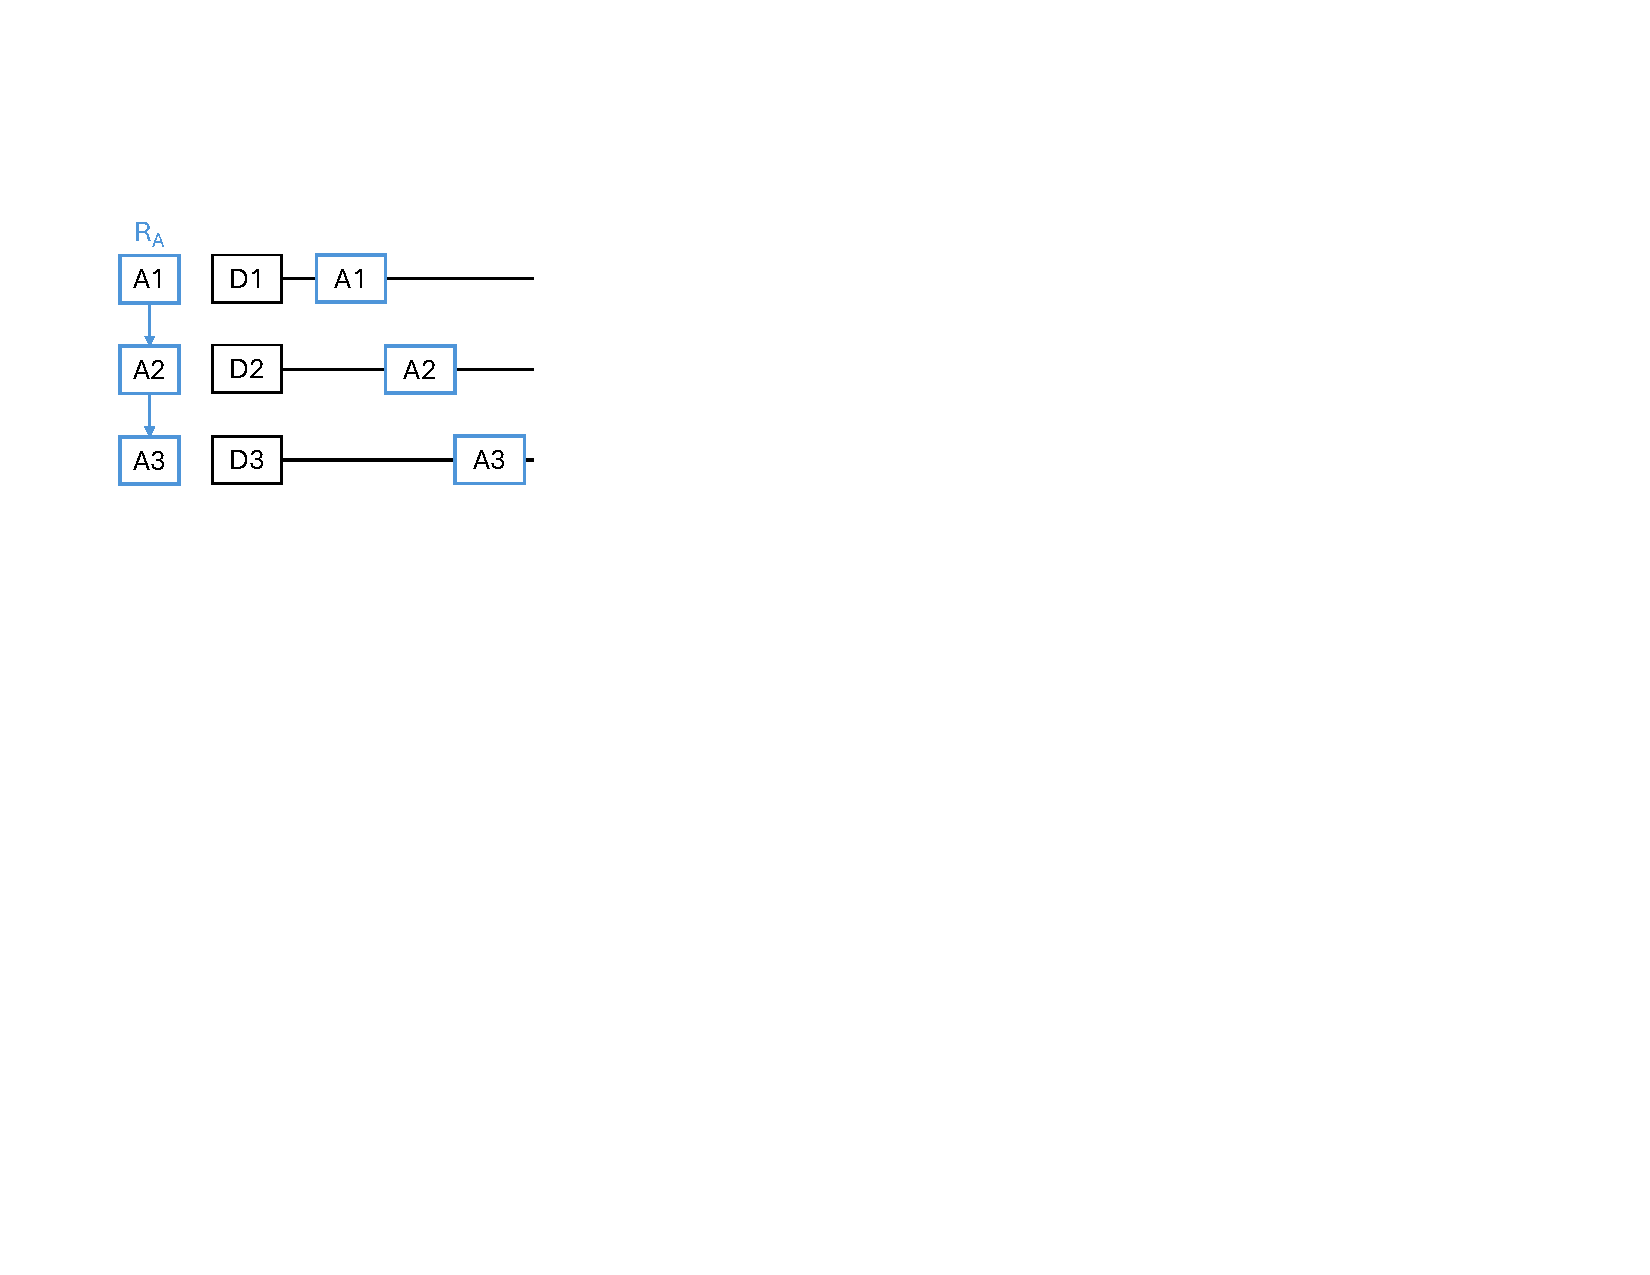
\includegraphics[width=\textwidth]{RASC/figures/applications/tl-vs-dag-tl/sched-ra.pdf}}
        \caption{\small $R_A$.}
        \medskip
        \label{rasc:fig:ra-sched}
    \end{subfigure}%
    % \hfill
    % \rule{1pt}{0.14\linewidth}
    \hfill
    \begin{subfigure}[t]{0.33\linewidth}
        % \vspace{0.2cm}
        {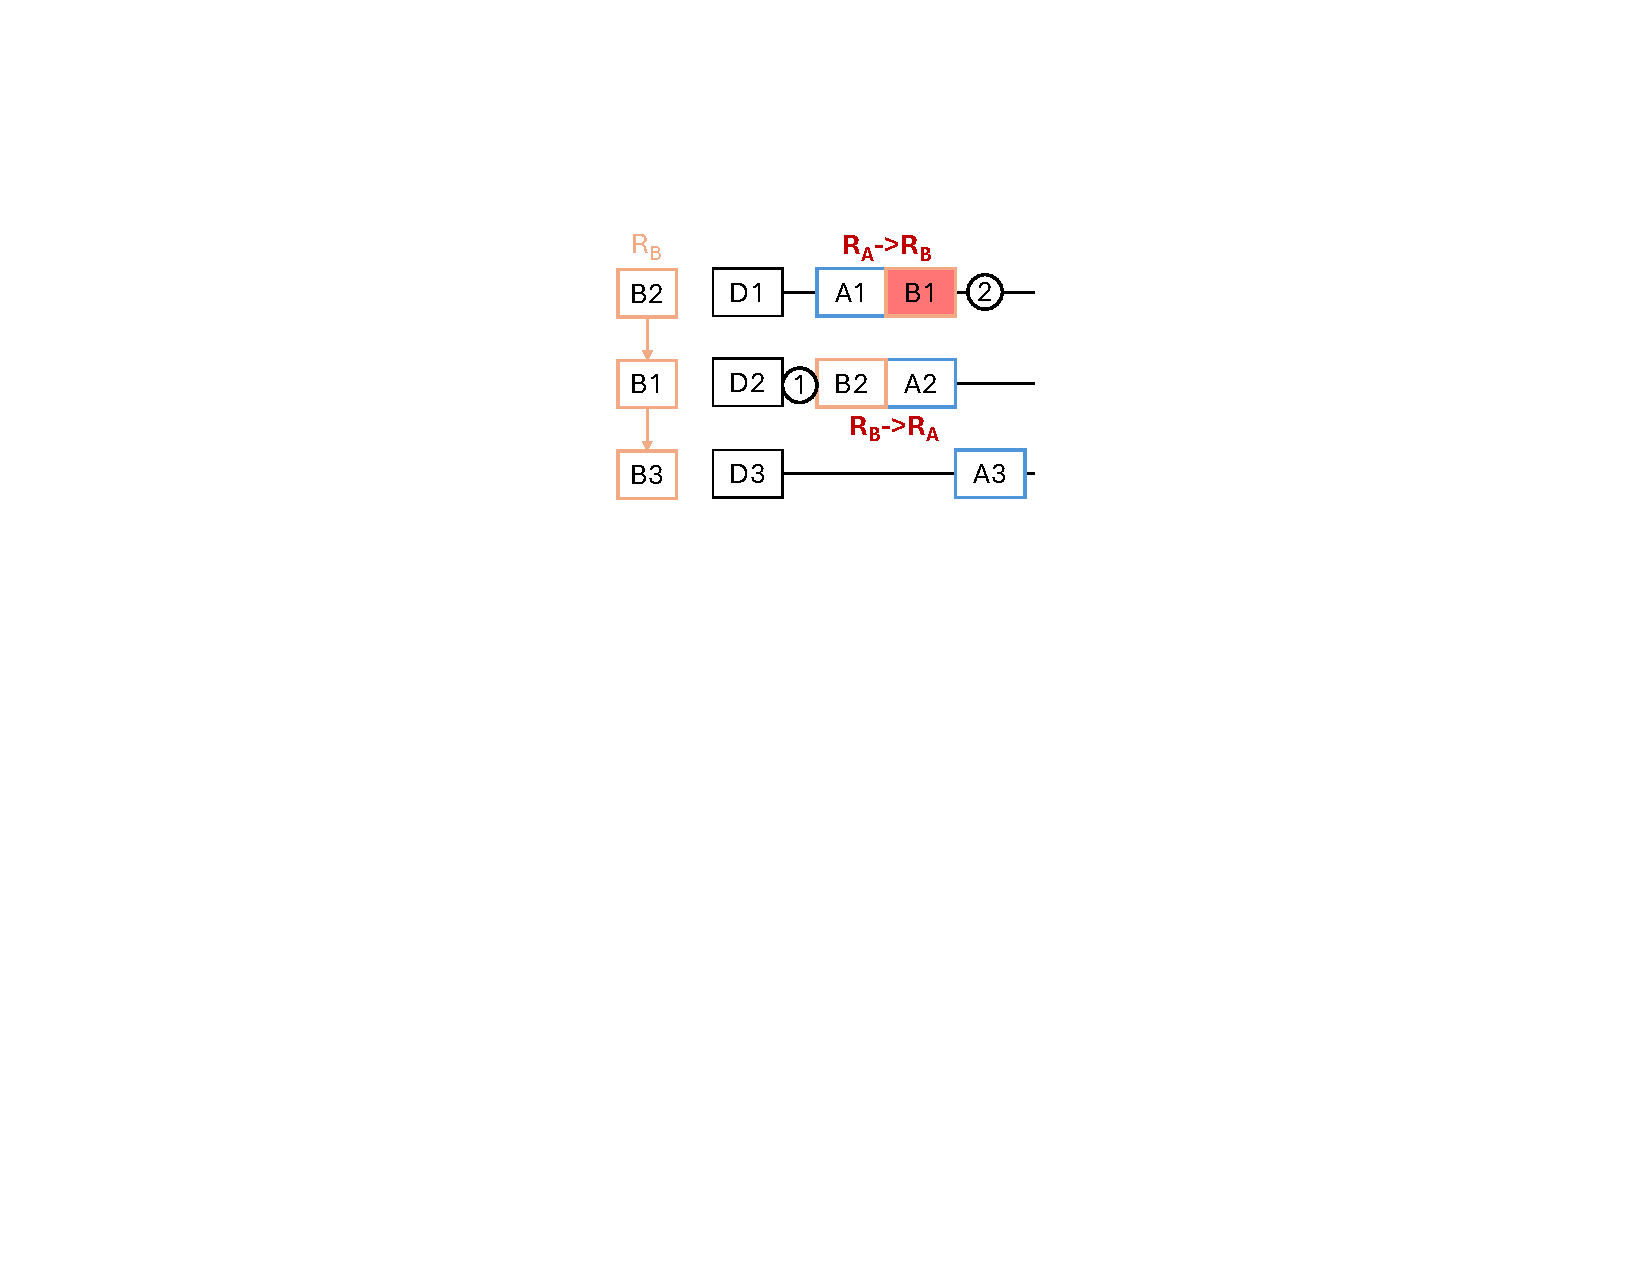
\includegraphics[width=\textwidth]{RASC/figures/applications/tl-vs-dag-tl/rb-tl-invalid.pdf}}
        \caption{\small $R_B$ \& invalid TL.}
        \medskip
        \label{rasc:fig:tl-invalid}
    \end{subfigure}%
    \hfill
    % \rule{1pt}{0.14\linewidth}
    % \hfill
    \begin{subfigure}[t]{0.32\linewidth}
        {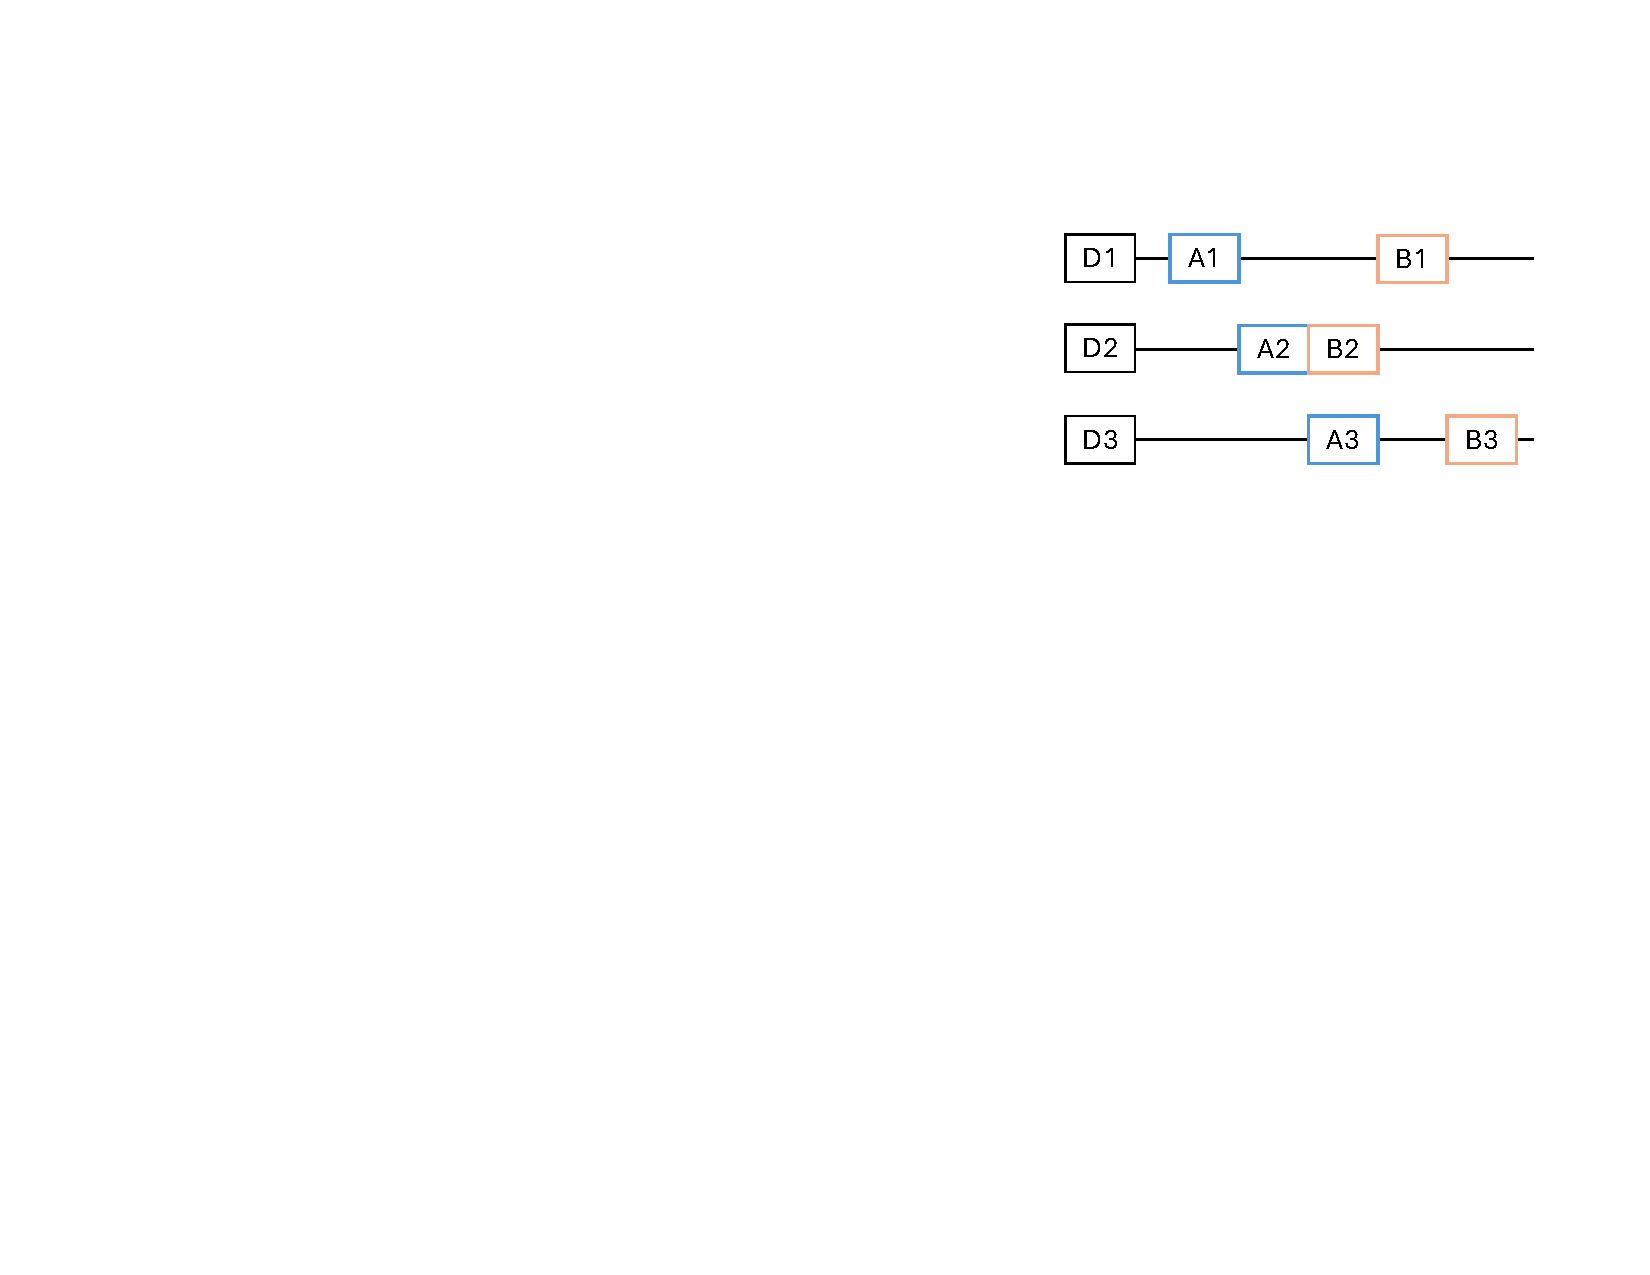
\includegraphics[width=\textwidth]{RASC/figures/applications/tl-vs-dag-tl/TL_valid.pdf}}
        \caption{\small $R_B$ \& valid TL.}
        \medskip
        \label{rasc:fig:tl-valid}
    \end{subfigure} 
    \par\medskip
    % \rule{1pt}{0.14\linewidth}
    % \hfill
    \begin{subfigure}[b]{0.35\linewidth}
        {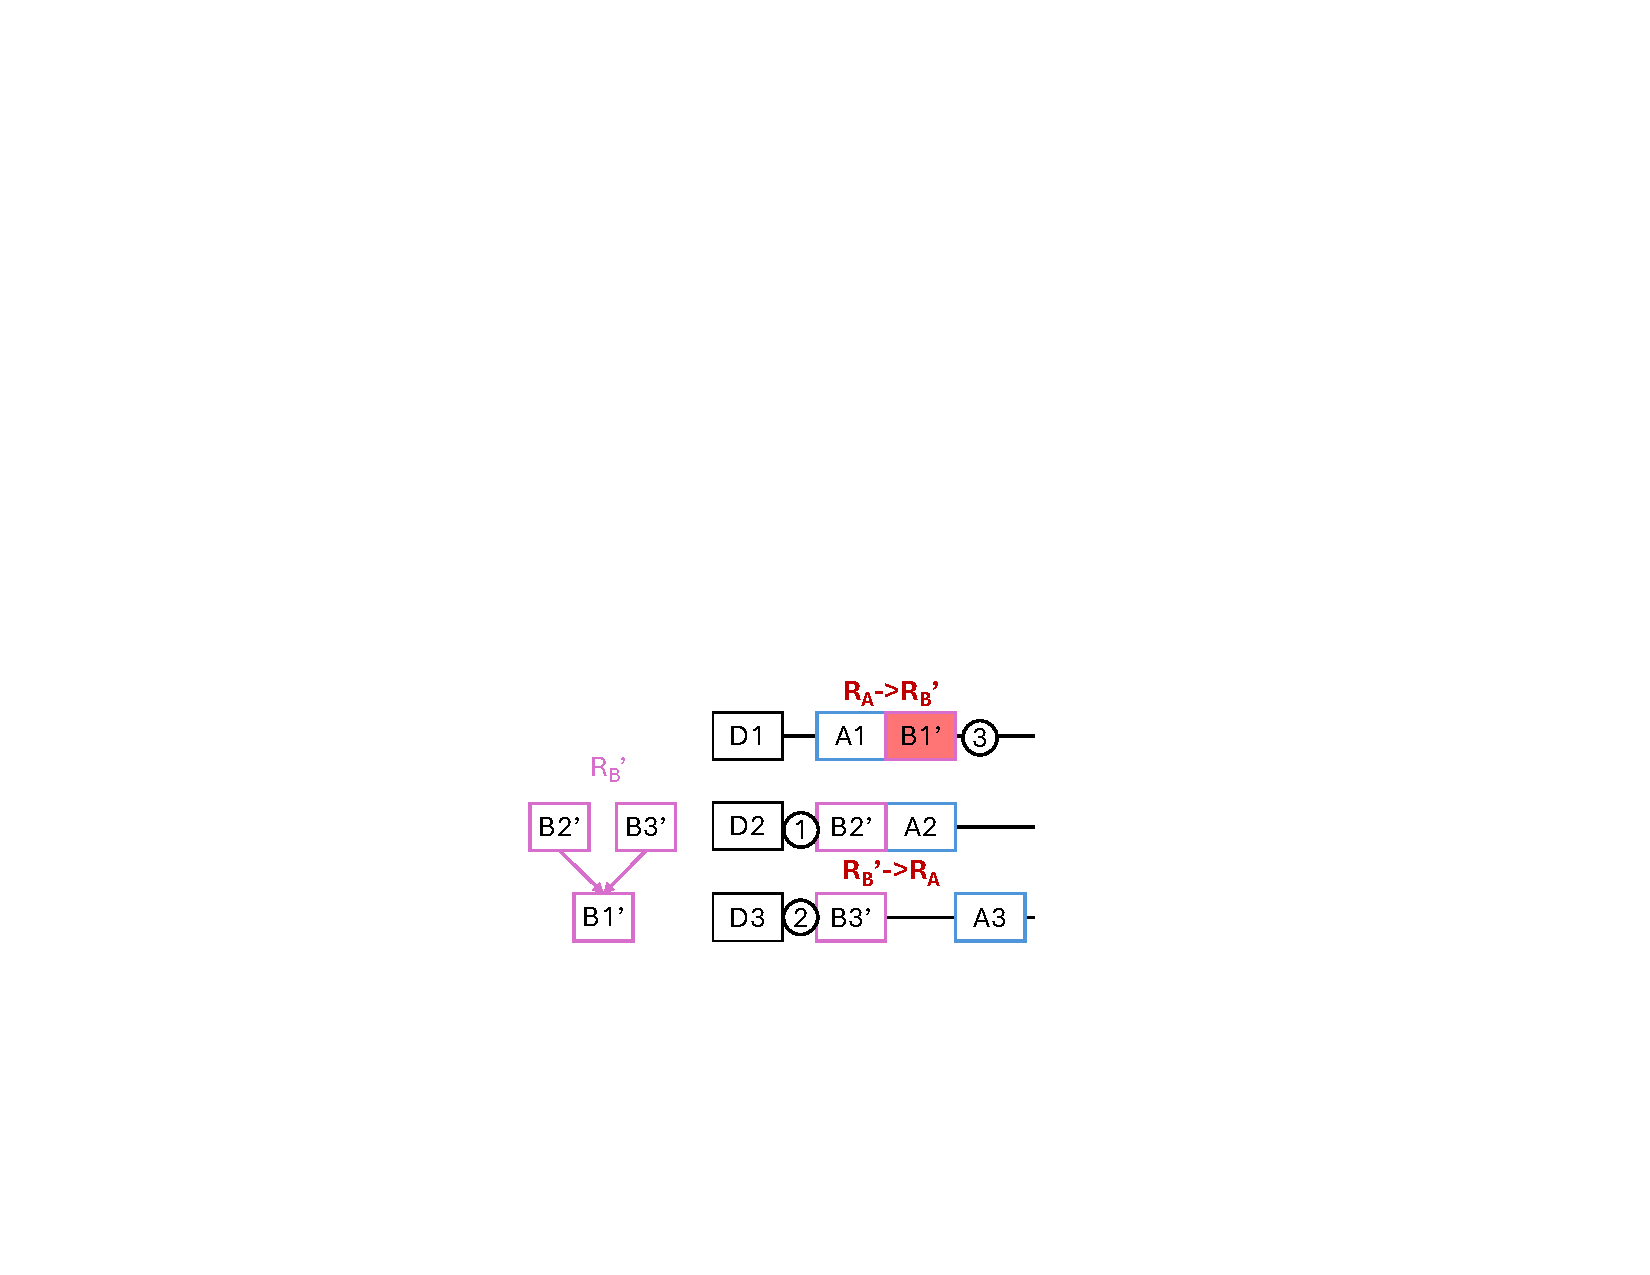
\includegraphics[width=\textwidth]{RASC/figures/applications/tl-vs-dag-tl/rb-dag-tl-invalid-new.pdf}}
        \caption{\small $R_B'$ \& invalid \scheduler.}
        \medskip
        \label{rasc:fig:dag-tl-invalid}
    \end{subfigure}%
    \hspace{0.02\linewidth}
    % \rule{1pt}{0.14\linewidth}
    % \hfill
    \begin{subfigure}[b]{0.3\linewidth}
        \centering
        {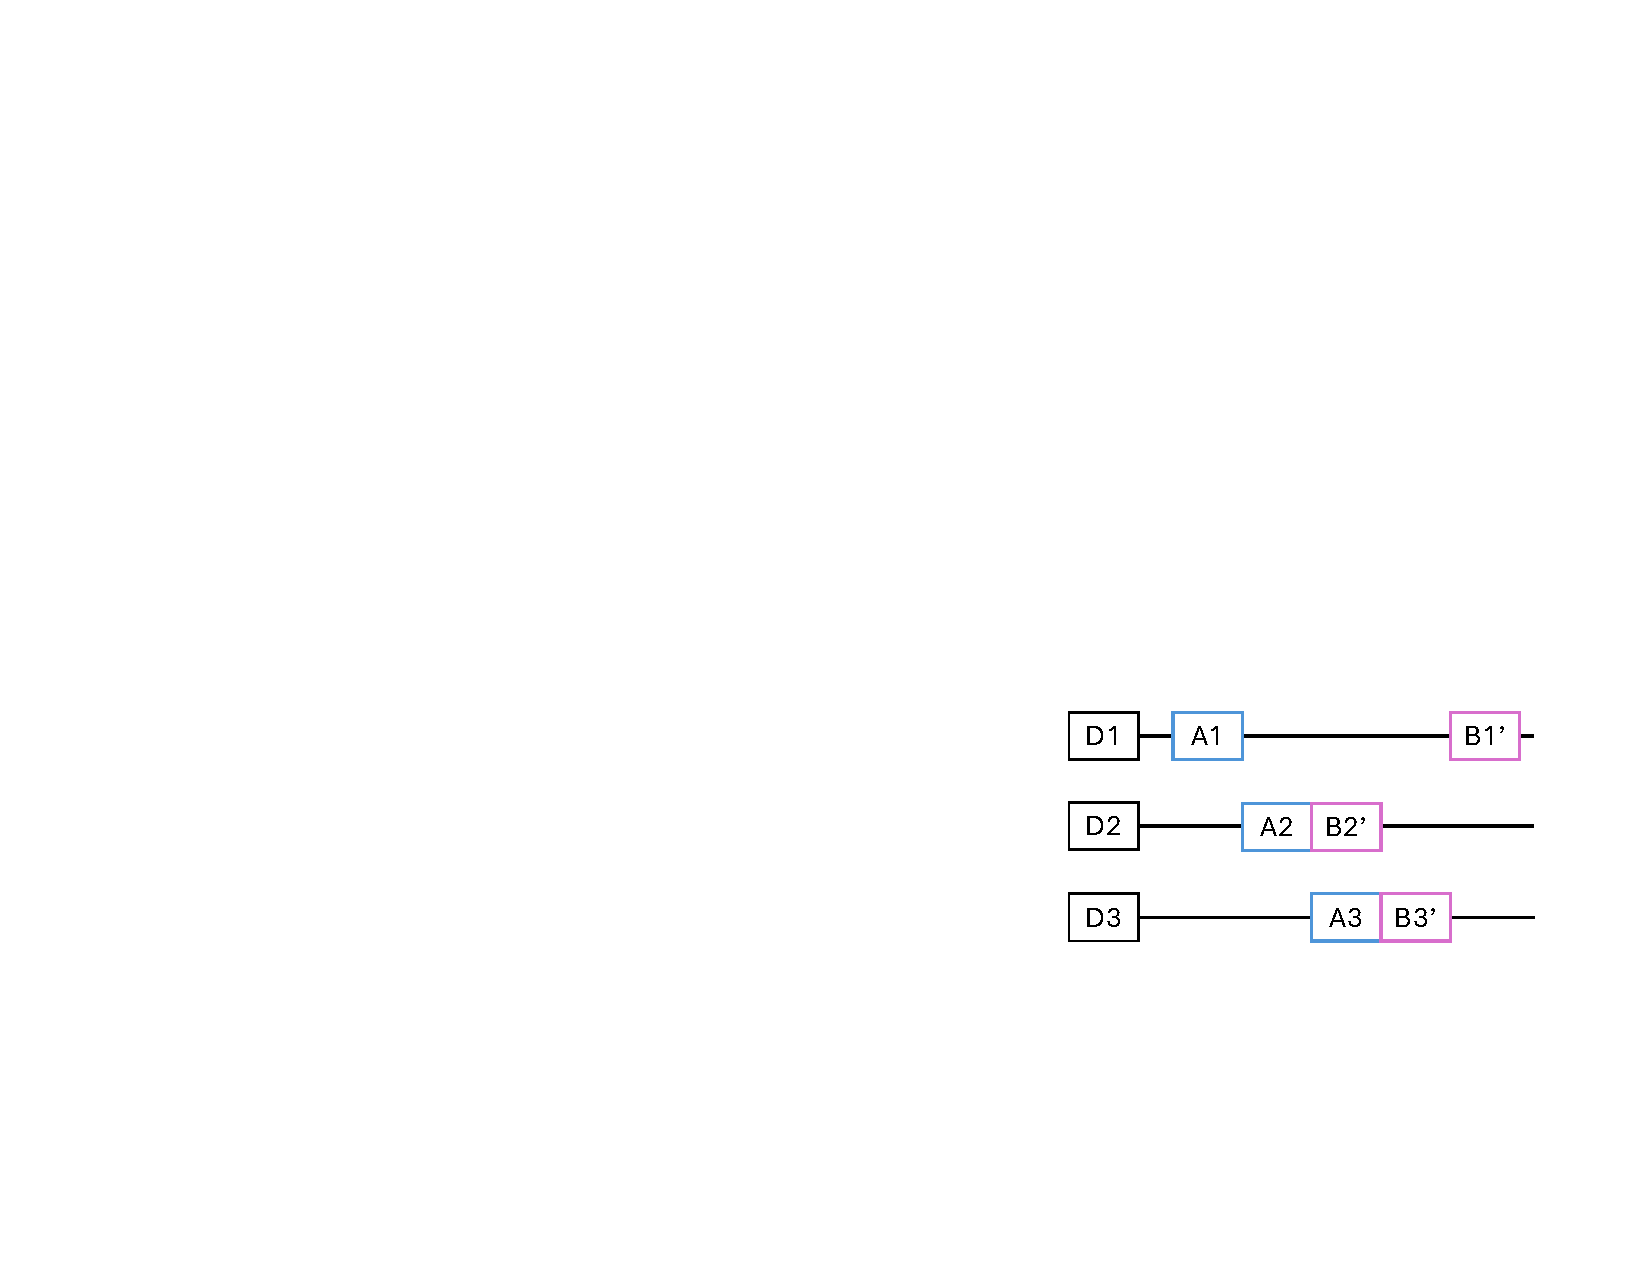
\includegraphics[width=\textwidth]{RASC/figures/applications/tl-vs-dag-tl/DAG-TL_valid-new.pdf}}
        \caption{\small $R_B'$ \& invalid \scheduler.}
        \medskip
        \label{rasc:fig:dag-tl-valid}
    \end{subfigure}
    % \hspace{0.1cm}
    
    \caption{\bf \small Example Routines and Schedule for TL vs \scheduler. {\it Action symbols feature a letter that stands for the routine they are a part of and a number to denote which device they execute on, e.g., $A1$ is part of routine $R_A$ and executes on device $D1$.}}
    \medskip
    \label{rasc:fig:TL-vs-DAG-TL}
\end{figure}

\subsubsection{Diverse Action-Causality Expressiveness}
\label{rasc:sec:causality}


Commercial IoT platforms rarely support cross-action dependencies: e.g., Alexa routines allow limited inter-routine chaining,\footnote{Alexa can call a routine from another but offers no richer dependencies.} but not dependencies between actions. The \abs{} abstraction enables both cross-action and finer-grained dependencies across critical points {\it inside} an action's progress.
\Cref{rasc:fig:energy-saving-vacuum-rasc,rasc:fig:garage-routine-workflow} depict {\it co-action} and \textit{fallback action} examples.

In \sysname{} each routine is represented internally as a DAG of device actions (\Cref{rasc:fig:energy-saving-vacuum-rasc}). When an action emits a progress event (A, S, or C), \sysname{} inspects its dependent children; any child whose dependencies are satisfied is immediately scheduled to run. \sysname{} execution is {\it event-driven}. 

\subsubsection{Dynamic Action Scheduling}
\label{rasc:sec:dyn-sched}

We describe how to schedule routines and actions when some of these actions take a shorter or longer time than expected. 

\noindent\textbf{Background.}
In real-world IoT deployments, action durations vary widely:
ovens heat faster when pre-warmed, elevators stall if doors are obstructed,
and HVAC cycles fluctuate with outside temperature. 
Due to these variable times, any static schedule that is made, which devices execute (to respect dependencies) will need to be {\it dynamically} adjusted at runtime.

The real-time systems community studied this problem through
\emph{resource reclamation algorithms}~\cite{shen1993resource,manimaran1997new,gupta2000new}.
These algorithms optimize for \emph{early completions}:
if a task finishes ahead of its worst-case bound, subsequent tasks can advance to reclaim idle time while maintaining precedence.
For example, \emph{Restriction Vectors (RV)}~\cite{manimaran1997new}
maintains a task timeline and, upon early task completion, pulls dependent tasks forward to begin once all predecessors have completed. This reclaims idle slack while preserving precedence constraints.

\noindent\textbf{Challenges.} 
We need to extend reclaiming algorithms to handle both early completions and 
actions \textit{exceeding} their schedule. 
A heater lagging on a cold day or a door closing slower than usual delays subsequent tasks, and naive scheduling
can break causal dependencies or stall routines. 

\sysname's fine-grained causality model (\Cref{rasc:sec:causality}) makes scheduling challenging:
we must honor dependencies at arbitrary progress points (e.g., Ack, Start, Complete), increasing potential conflicts and correctness risks.

Correct IoT scheduling hinges on two properties: \textbf{\textit{Safety}} (no device receives two action requests at once) and \textbf{\textit{Serial Equivalence}} (overlapping routines execute with some serial order). Without them, final states can be unpredictable or inconsistent with any one routine. SafeHome~\cite{SafeHomeEuroSys2021} guarantees these only for fixed action durations.
However, with unpredictable durations and fine-grained dependencies, maintaining these guarantees requires adaptation.

\noindent\textbf{Overview.} 
\sysname{} extends reclamation-style scheduling to IoT,
building atop the \abs{} abstraction (\Cref{rasc:sec:rasc}).
\sysname's scheduling occurs in two phases: 
(i)~it schedules arriving routines (\Cref{rasc:sec:scheduler}), and
(ii)~it dynamically adjusts the schedule for early state changes and delays (\Cref{rasc:sec:rescheduler}). 
We present \textbf{\textit{DAG-TL}}, to ensure serial equivalence for routines despite variable action lengths, 
alongside two rescheduling policies, \textbf{\textit{STF and RV}}, which 
adapt to both early and late state changes while preserving
Safety and Serial Equivalence.


\subsubsubsection{\scheduler: Ensuring Routine Serial Equivalence}
\label{rasc:sec:scheduler}

We adapt the Timeline Scheduler (TL) from \cite{SafeHomeEuroSys2021}. 
Upon routine arrival, the original TL places actions in the earliest gaps that preserve 
intra-routine action order and inter-routine serialization order.
TL uses action-by-action backtracking to find gaps that
maintain serialization at all times.
For \sysname-style DAGs, the original TL has exponential worst-case time complexity. 

To handle \sysname-style routines expressed as DAGs, our {\it \scheduler} approach 
adopts an {\it aggressive backtrack strategy} that makes ``big jumps'' in the state space.
Specifically, upon detecting a serialization conflict, it jumps to the routine's top-level action and shifts the entire DAG forward in a single step---placing it after the last conflicting time found by inspecting the intersection of the preceding and following routine sets in the serialization order. By pruning unsatisfied paths early, we avoid repeated local retries.

\noindent\textbf{Illustrative example.}
\Cref{rasc:fig:TL-vs-DAG-TL} shows three routines: $R_A$, $R_B$ and $R_B'$. After sequential $R_A$ is scheduled (\Cref{rasc:fig:ra-sched}), sequential $R_B$ arrives.
TL fills the earliest gaps: it tentatively places $B2$ (1), then places $B1$ (2), which reveals a serialization violation (\Cref{rasc:fig:tl-invalid}).
TL then moves $B2$ after $A2$ (the next available gap) and completes scheduling $R_B$ without further violations (\Cref{rasc:fig:tl-valid}).
Now consider non-sequential $R_B'$ arriving after $R_A$ (\Cref{rasc:fig:dag-tl-invalid}). 
Here $B1'$ depends on $B2'$ and $B3'$.
With a breadth-first traversal, \scheduler{} encounters a violation at the third step ($B1'$); it schedules $R_B'$ anew from the root and shifts the entire DAG so that all of $R_B'$ follows $R_A$ on any shared device (\Cref{rasc:fig:dag-tl-valid}). 
Naïve per-conflict backtracking would recheck and reschedule many prior actions and does not scale; \scheduler's top-level backtrack reduces scheduling steps in practice.

\subsubsubsection{Rescheduler}
\label{rasc:sec:rescheduler}


An action may finish later (over-time) or earlier (under-time) than initially scheduled. \sysname{} must adjust. 
We describe how actions are rescheduled to accommodate schedule deviations, 
while minimizing routine completion time and continuing to ensure safety, serial equivalence, and performance. 

\noindent \textbf{\underline{Problem Statement}. }
Each routine $R$ is a DAG of actions. An action $a$ has:
(i) a device $dev(a)$,
(ii) a (possibly data-driven) duration estimate $len(a)$, and
(iii) dependency edges to its parents in the routine $Pred_{\text{DAG}}(a)$.
Multiple routines may run concurrently and touch overlapping device sets.

Our goal is to maintain a {\it feasible schedule} that (1) is \textbf{Safe} (no device runs two actions at once), (2) is \textbf{Serially Equivalent}~\cite{SafeHomeEuroSys2021}  across routines (the final state equals some serial execution of whole routines), and (3) \textbf{adapts} when actions finish early/late while preserving (1)-(2).

\noindent \textbf{{When to Trigger the Rescheduler}. }
Late actions are handled by \sysname{} {\it proactively}, to ensure safety. When a high percentage of the action's state change length upper bound $U$ (\Cref{rasc:sec:adaptive-polling-strategy}) has elapsed (95\% in our implementation), \sysname{} extrapolates to estimate the new state change time (e.g., oven took 20 min to warm up from 200\textdegree F to 400\textdegree F, then \sysname{} estimates it will take 5 min more to get to the target 450\textdegree F). 

Early-state-changing actions are handled
{\it reactively}, as early state changes do not violate safety. If the difference between expected and actual state change exceeds a threshold (1 s in implementation), we invoke the rescheduler. 

\noindent \textbf{{Constraints on the Rescheduler}. } 
Rescheduling must respect two primary constraints: (1) dependency on prior actions in a routine, and (2) the (immutable) serialization order established (\Cref{rasc:sec:scheduler}) across active routines. We handle these via preprocessing and two specialized rescheduling algorithms. 

\noindent \textbf{{Preprocessing}.}
Let $\mathcal{I}$ be the set of potentially impacted actions. 
We add an action $A'$ to $\mathcal{I}$ when a deviation on action $A$ satisfies any one of three conditions:
(i) $A'$ is in the same routine $R$ and is a descendant of $A$ in $R$'s action DAG;
(ii) $A'$ is scheduled to start after $A$ on the same device $D$ that deviated;
(iii) $A'$ belongs to a routine $R'$ that is serialized after $R$.

To preserve the \emph{established} serial order among routines, \sysname{} records each routine's \emph{postset}: the routines that, on any shared device, have executed after it up to the rescheduler's trigger time. It then constructs an immutable serialization order by repeatedly: (1) selecting all routines with empty postsets, (2) placing them at the front of the order (breaking ties by arrival time), and (3) removing them from the remaining postsets. We iterate until all routines are placed.

\begin{figure}[th]
  \centering

  % Row 1
  \begin{subfigure}[b]{0.41\linewidth}
    \centering
    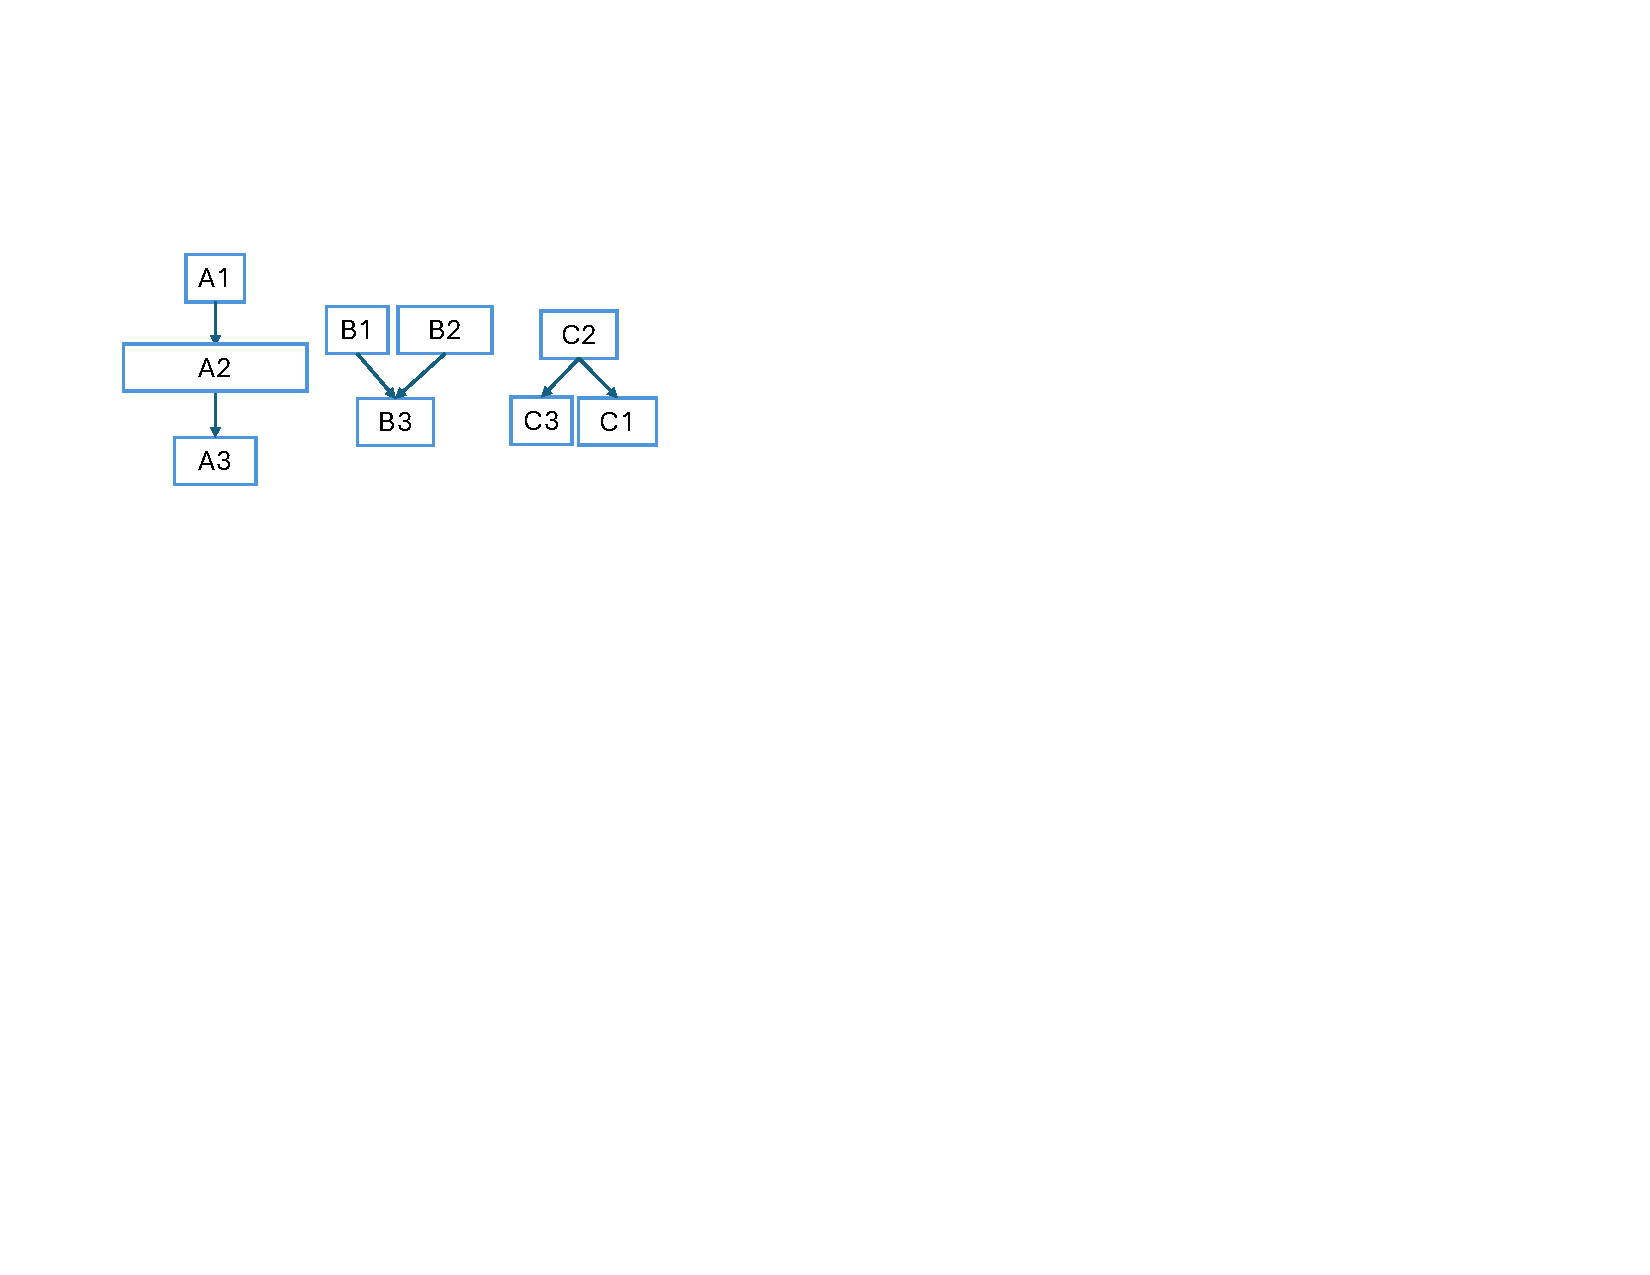
\includegraphics[width=0.9\textwidth]{RASC/figures/applications/Reschedule_routines.pdf}
    \bigskip
    \caption{\small Routine graphs.}
    \label{rasc:fig:resched-routines}
  \end{subfigure}
  \hspace{0.5cm}
  \begin{subfigure}[b]{0.41\linewidth}
    \centering
    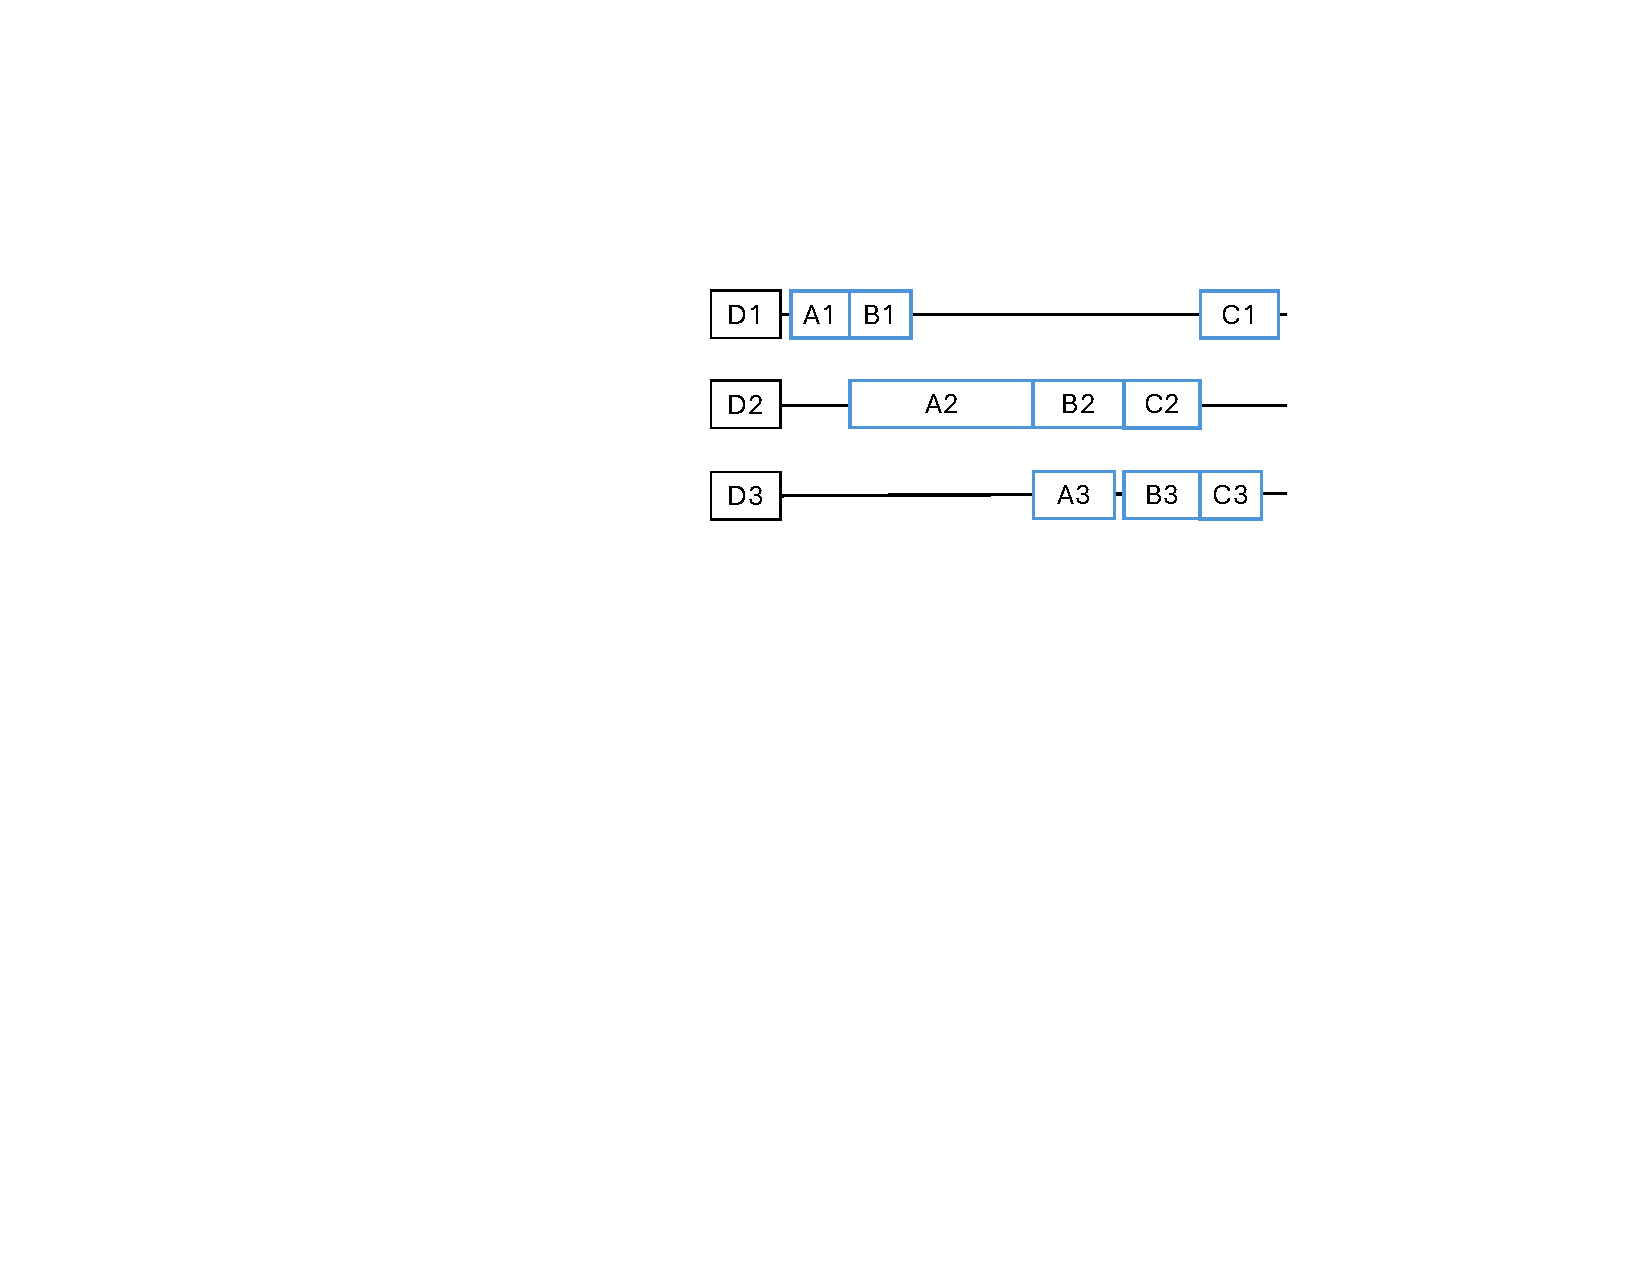
\includegraphics[width=\textwidth]{RASC/figures/applications/Reschedule_og_schedule.pdf}
    \caption{\small Original schedule.}
    \label{rasc:fig:resched-og-sched}
  \end{subfigure}

  \par\medskip

  % Row 2
  \begin{subfigure}[b]{0.41\linewidth}
    \centering
    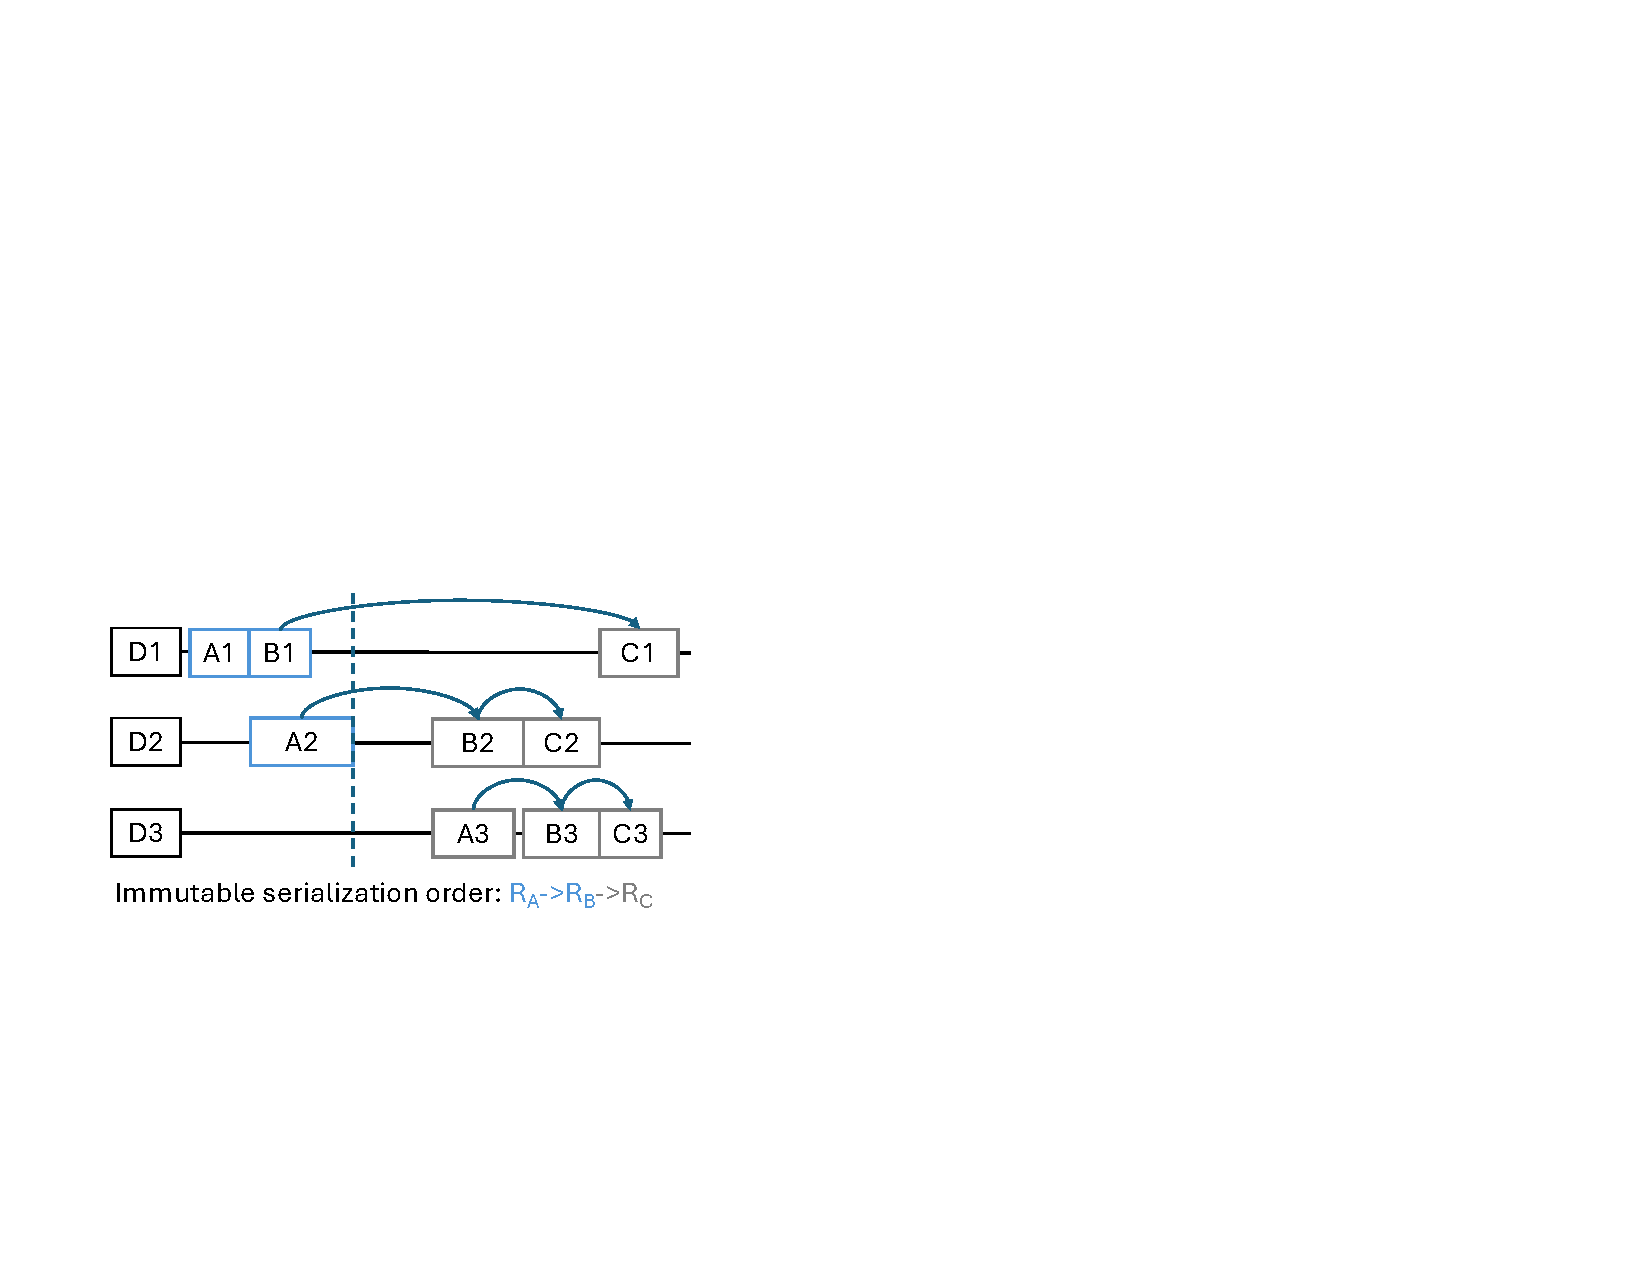
\includegraphics[width=\textwidth]{RASC/figures/applications/Reschedule_a2_end.pdf}
    \caption{\small Preprocessing phase.}
    \label{rasc:fig:resched-a2-end}
  \end{subfigure}
  % \hfill
  \hspace{0.5cm}
  \begin{subfigure}[b]{0.41\linewidth}
    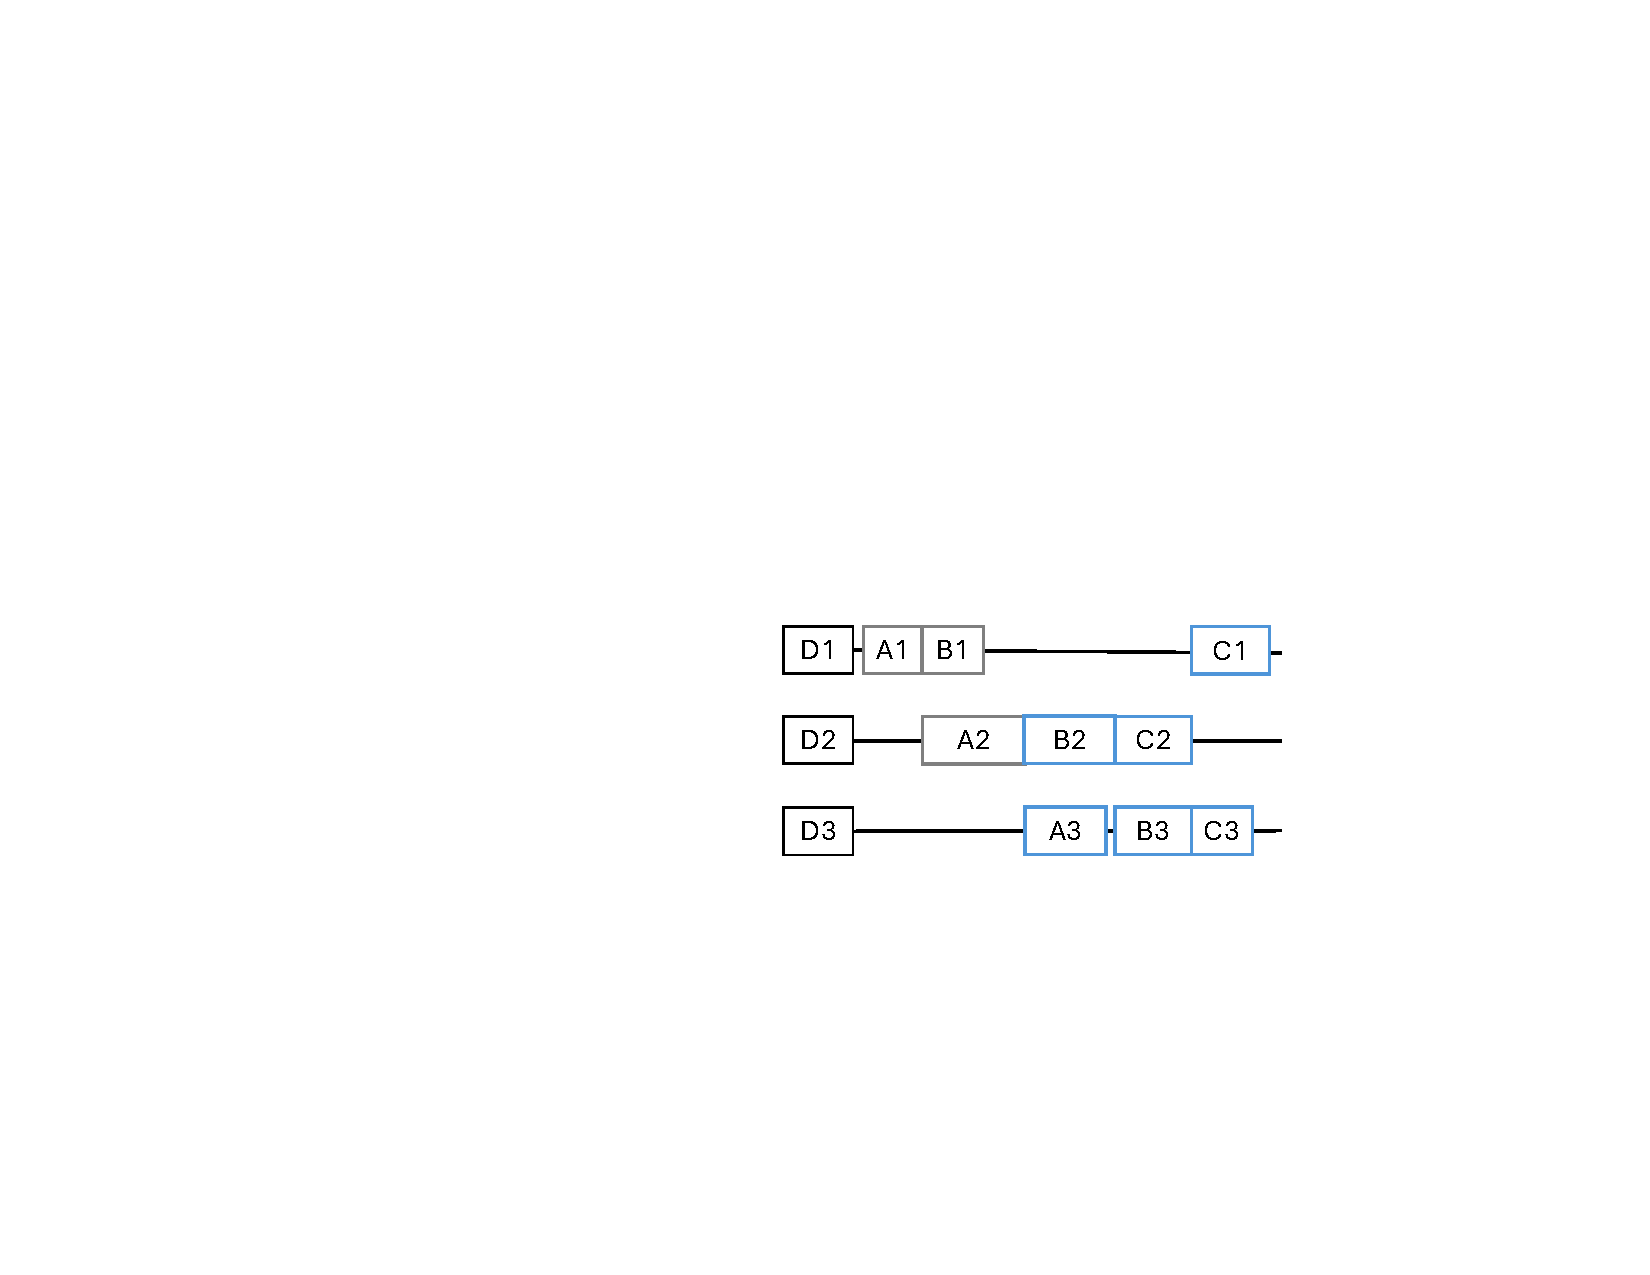
\includegraphics[width=0.83\textwidth]{RASC/figures/applications/Reschedule_sjfw_out.pdf}
    \caption{\small Rescheduling phase.}
    \label{rasc:fig:resched-sjfw-out}
  \end{subfigure}

  \caption{\small \textbf{Rescheduling in \sysname:} Example Routines.}
  \medskip
  \label{rasc:fig:resched}
\end{figure}


\sysname{} deschedules all actions in $\mathcal{I}$, and reschedules them while still preserving the established serial order.
For the routines in \Cref{rasc:fig:resched-routines} and the original \scheduler{} schedule in \Cref{rasc:fig:resched-og-sched}, \Cref{rasc:fig:resched-a2-end} shows the case where $A2$ completes early: affected actions (grey) are descheduled, the immutable order is $R_A\!\rightarrow\!R_B$, and routines that have not yet started (e.g., $R_C$) are left unchanged. Finally, \sysname{} inserts cross-routine, same-device dependencies to maintain serial equivalence. 

\begin{algorithm}[t]
    \caption{\bf Shortest Task First (STF) with Serializability}
    \label{rasc:algo:sjfw}
    \footnotesize
    \algtext*{EndIf} % hide EndIf but keep block structure
    \algtext*{EndElse} % same for Else
    \algtext*{EndFor} % same for For
    \algtext*{EndWhile} % same for For
    \begin{algorithmic}[1]
    \Require Impacted actions $\mathcal{A}$; duration $len(a)$; device $dev(a)$;
             routine DAG predecessors $Pred_{\text{DAG}}(a)$; immutable routine order $\prec$;
             device next-free times $next\_free[d]$ from current schedule.
    \Ensure Updated schedule without violating device safety or serial equivalence.
    
    \Statex \textbf{Phase 0: Add serialization edges (once).}
    \ForAll{pairs of routines $R \prec R'$}
      \ForAll{devices $d$ shared by $R$ and $R'$}
        \State Add edge from last action of $R$ on $d$ to first action of $R'$ on $d$
      \EndFor
    \EndFor
    
    \Statex \textbf{Phase 1: Initialize readiness and earliest feasible starts.}
    \ForAll{$a \in \mathcal{A}$}
      \State $Pred(a) \gets Pred_{\text{DAG}}(a) \cup Pred_{\text{serial}}(a)$
      \State $indeg[a] \gets |Pred(a)|$; \ $EST[a] \gets 0$; \ $FIN[a] \gets \text{unset}$
    \EndFor
    \State $Ready \gets \{ a \in \mathcal{A} \mid indeg[a]=0 \}$
    \ForAll{$a \in Ready$}
      \State $start\_cand[a] \gets next\_free[dev(a)]$
    \EndFor
    
    \Statex \textbf{Phase 2: List scheduling (single priority queue).}
    \While{$Ready \neq \emptyset$}
      \State $a^\star \gets \arg\min_{a \in Ready} \ (start\_cand[a], len(a))$ \Comment{Earliest start, then shortest task}
      \State $s \gets start\_cand[a^\star]$; \ $f \gets s + len(a^\star)$
      \State Place $a^\star$ on timeline of $dev(a^\star)$ at $[s,f)$
      \State $FIN[a^\star] \gets f$; \ $next\_free[dev(a^\star)] \gets f$
      \State Remove $a^\star$ from $Ready$
      \ForAll{successors $b$ of $a^\star$ in $Pred(\cdot)$}
        \State $indeg[b] \gets indeg[b]-1$
        \State $EST[b] \gets \max(EST[b], \ FIN[a^\star])$
        \If{$indeg[b]=0$}
          \State $start\_cand[b] \gets \max(EST[b], next\_free[dev(b)])$
          \State Insert $b$ into $Ready$
        \EndIf
      \EndFor
    \EndWhile
    \State \textbf{return} updated schedule
\end{algorithmic}
\end{algorithm}

\noindent \textbf{{Rescheduling}.} We reschedule descheduled actions using two policies.
First, we augment the Shortest Task First (STF) algorithm (known to be optimal~\cite{Tanenbaum2006}) to honor inter- and intra-routine dependencies
(\Cref{rasc:algo:sjfw}). 
We prioritize actions 
by estimated length; we repeatedly (i) pick the head, (ii) place it in the earliest common free slot across required devices, and (iii) update downstream dependencies, until the queue empties.
In \Cref{rasc:fig:resched}, STF respects the immutable serialization order, not placing $C2$ before $B2$ despite $C2$ being shorter (\Cref{rasc:fig:resched-sjfw-out}).

\begin{figure}[t!]
    \begin{subfigure}[t]{0.18\linewidth}
        \centering
        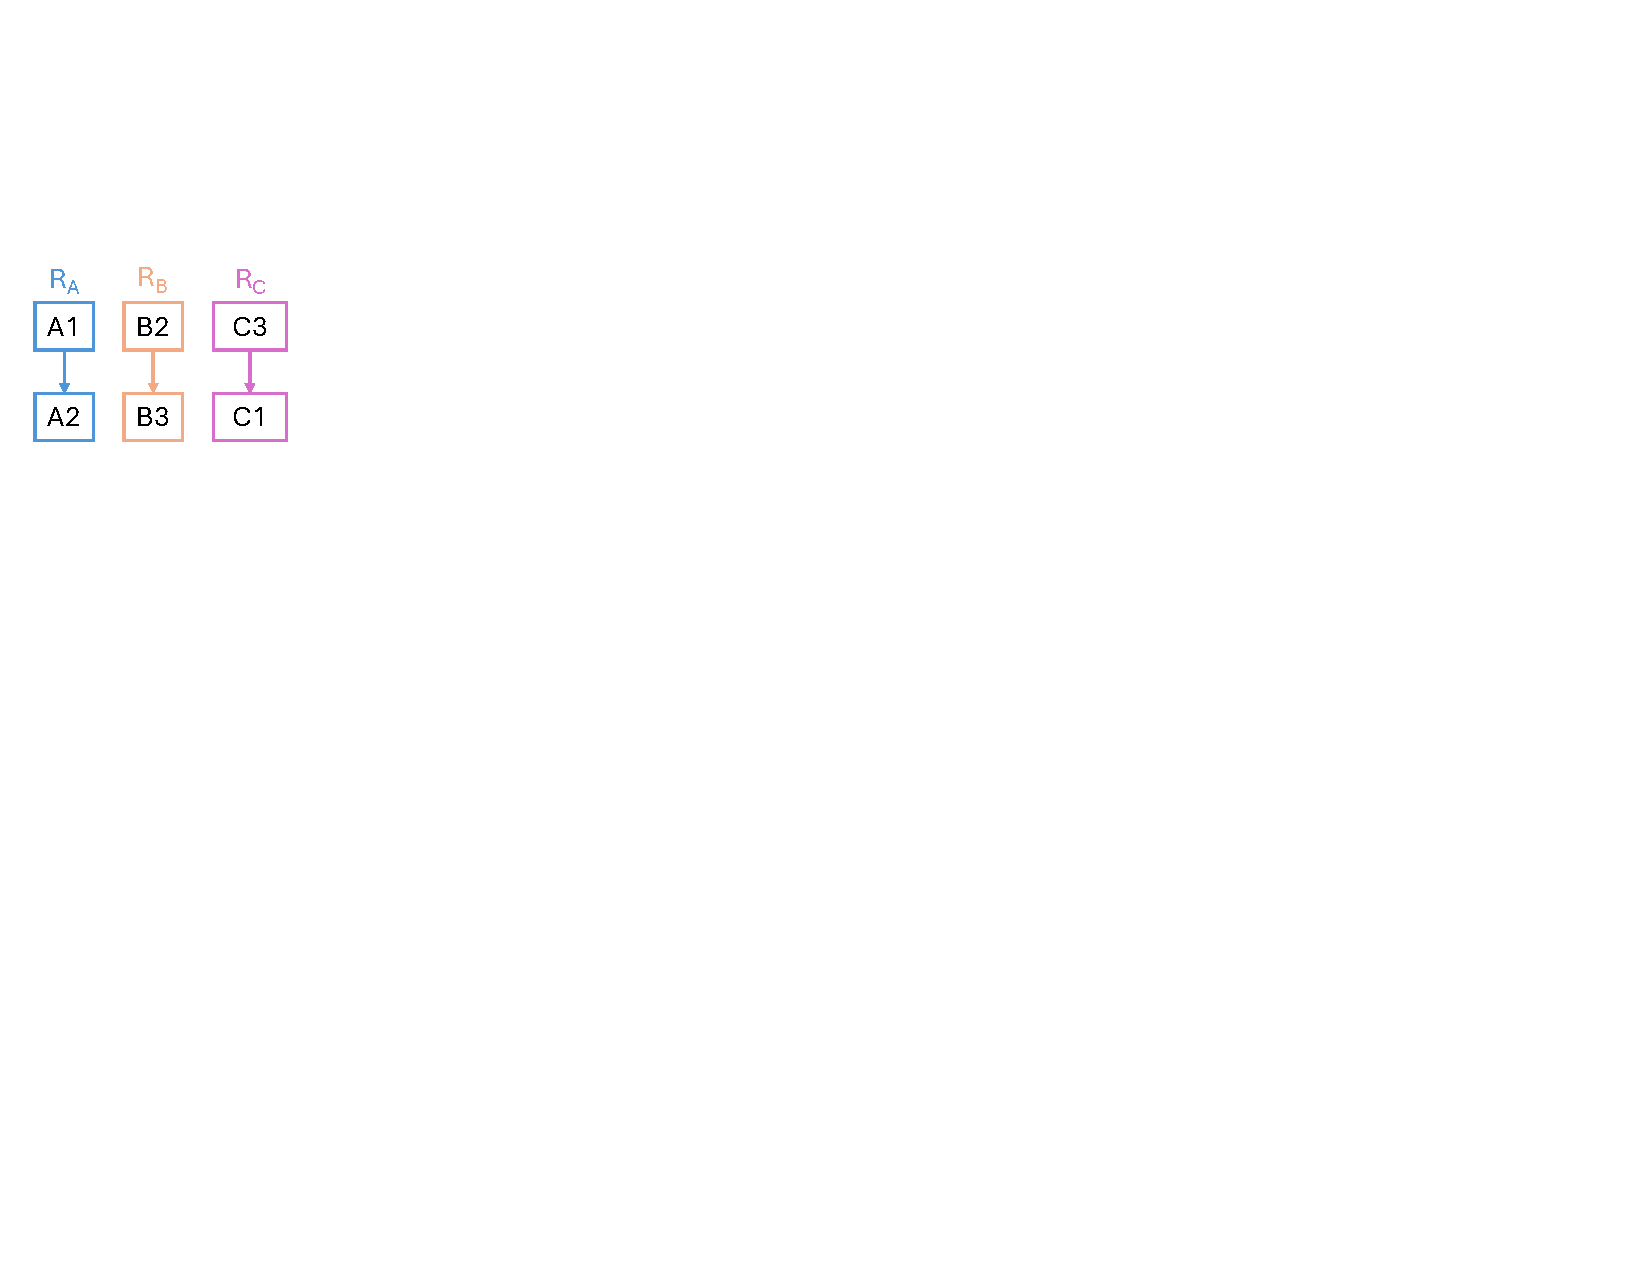
\includegraphics[width=\linewidth]{RASC/figures/applications/RASCal RV a.pdf}
        \caption{\small Routine graphs.}
        \medskip
        \label{rasc:fig:rv-graphs}
    \end{subfigure}
    \hfill
    \begin{subfigure}[t]{0.26\linewidth}
        \centering
        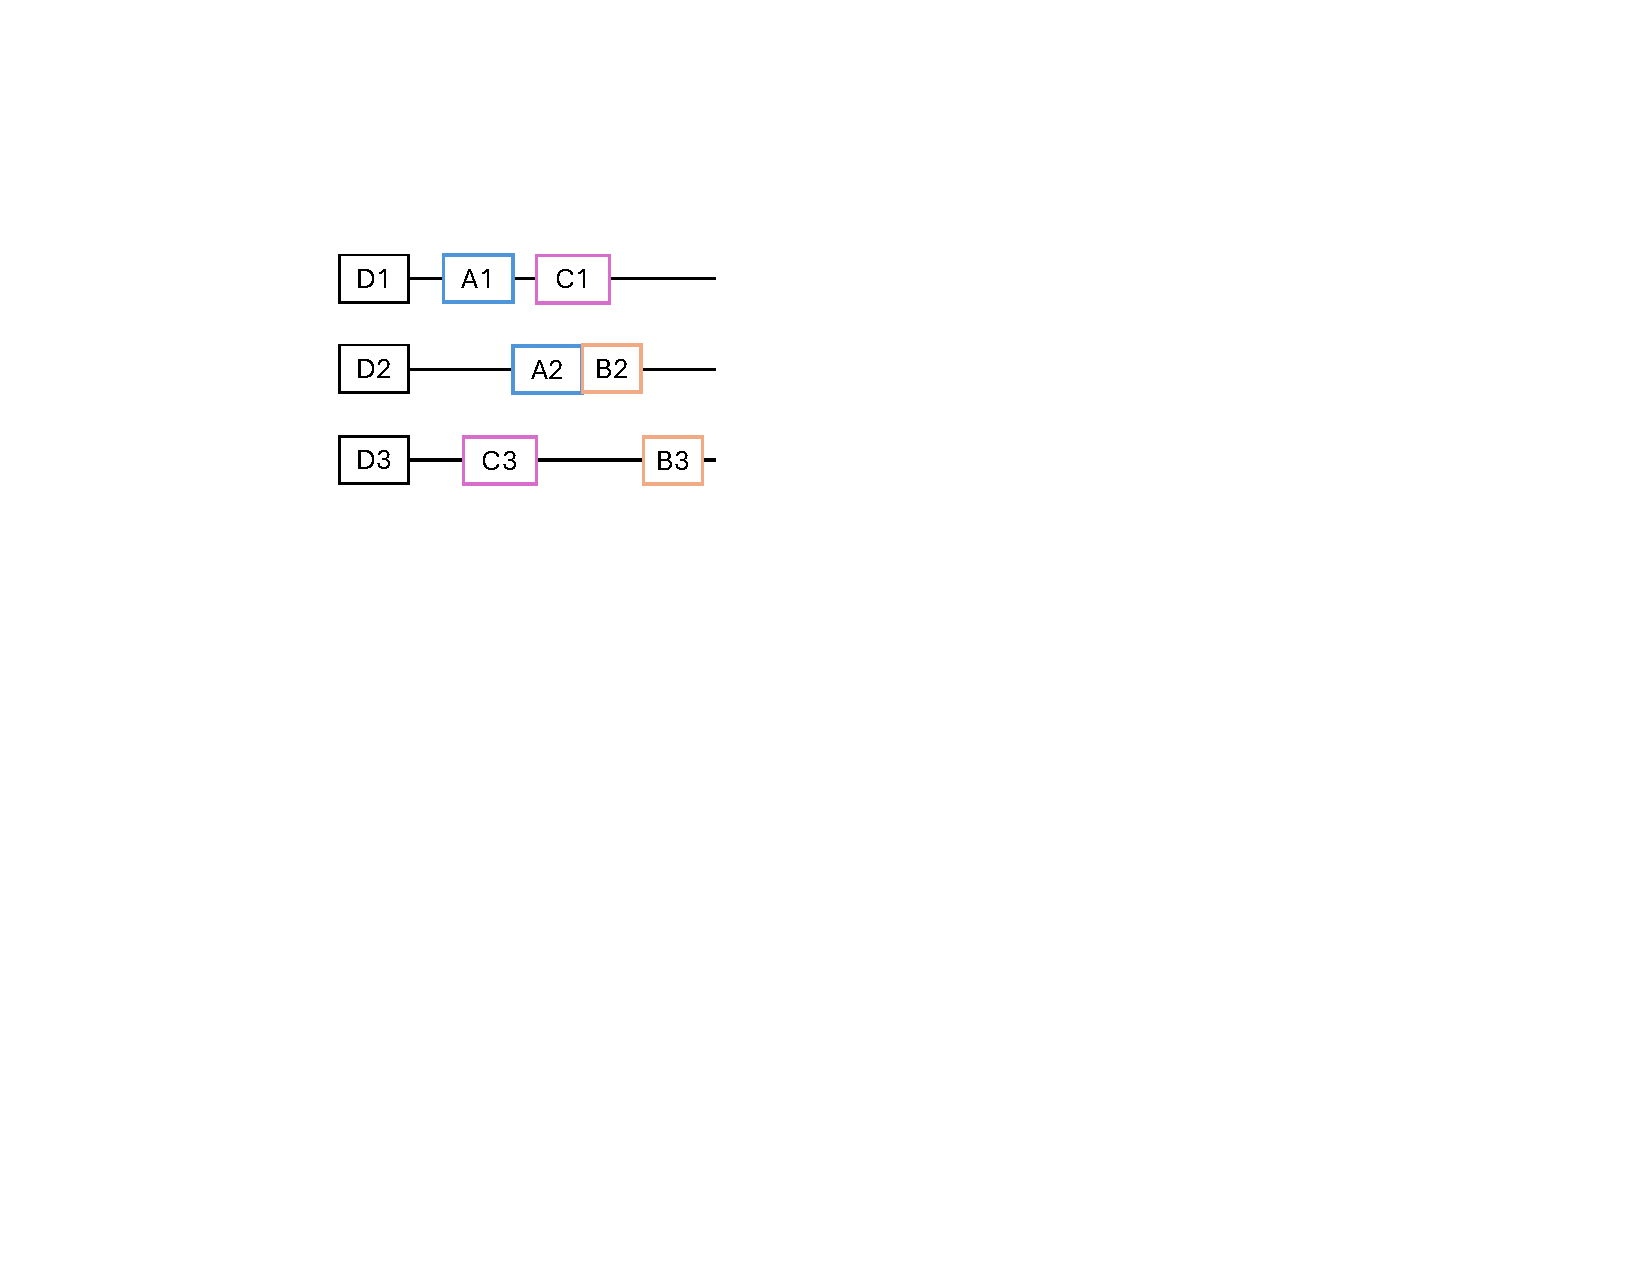
\includegraphics[width=\linewidth]{RASC/figures/applications/RASCal RV b.pdf}
        \caption{\small Original \scheduler{} schedule.}
        \medskip
        \label{rasc:fig:rv-dag-tl}
    \end{subfigure}
    \hfill
    \begin{subfigure}[t]{0.25\linewidth}
        \centering
        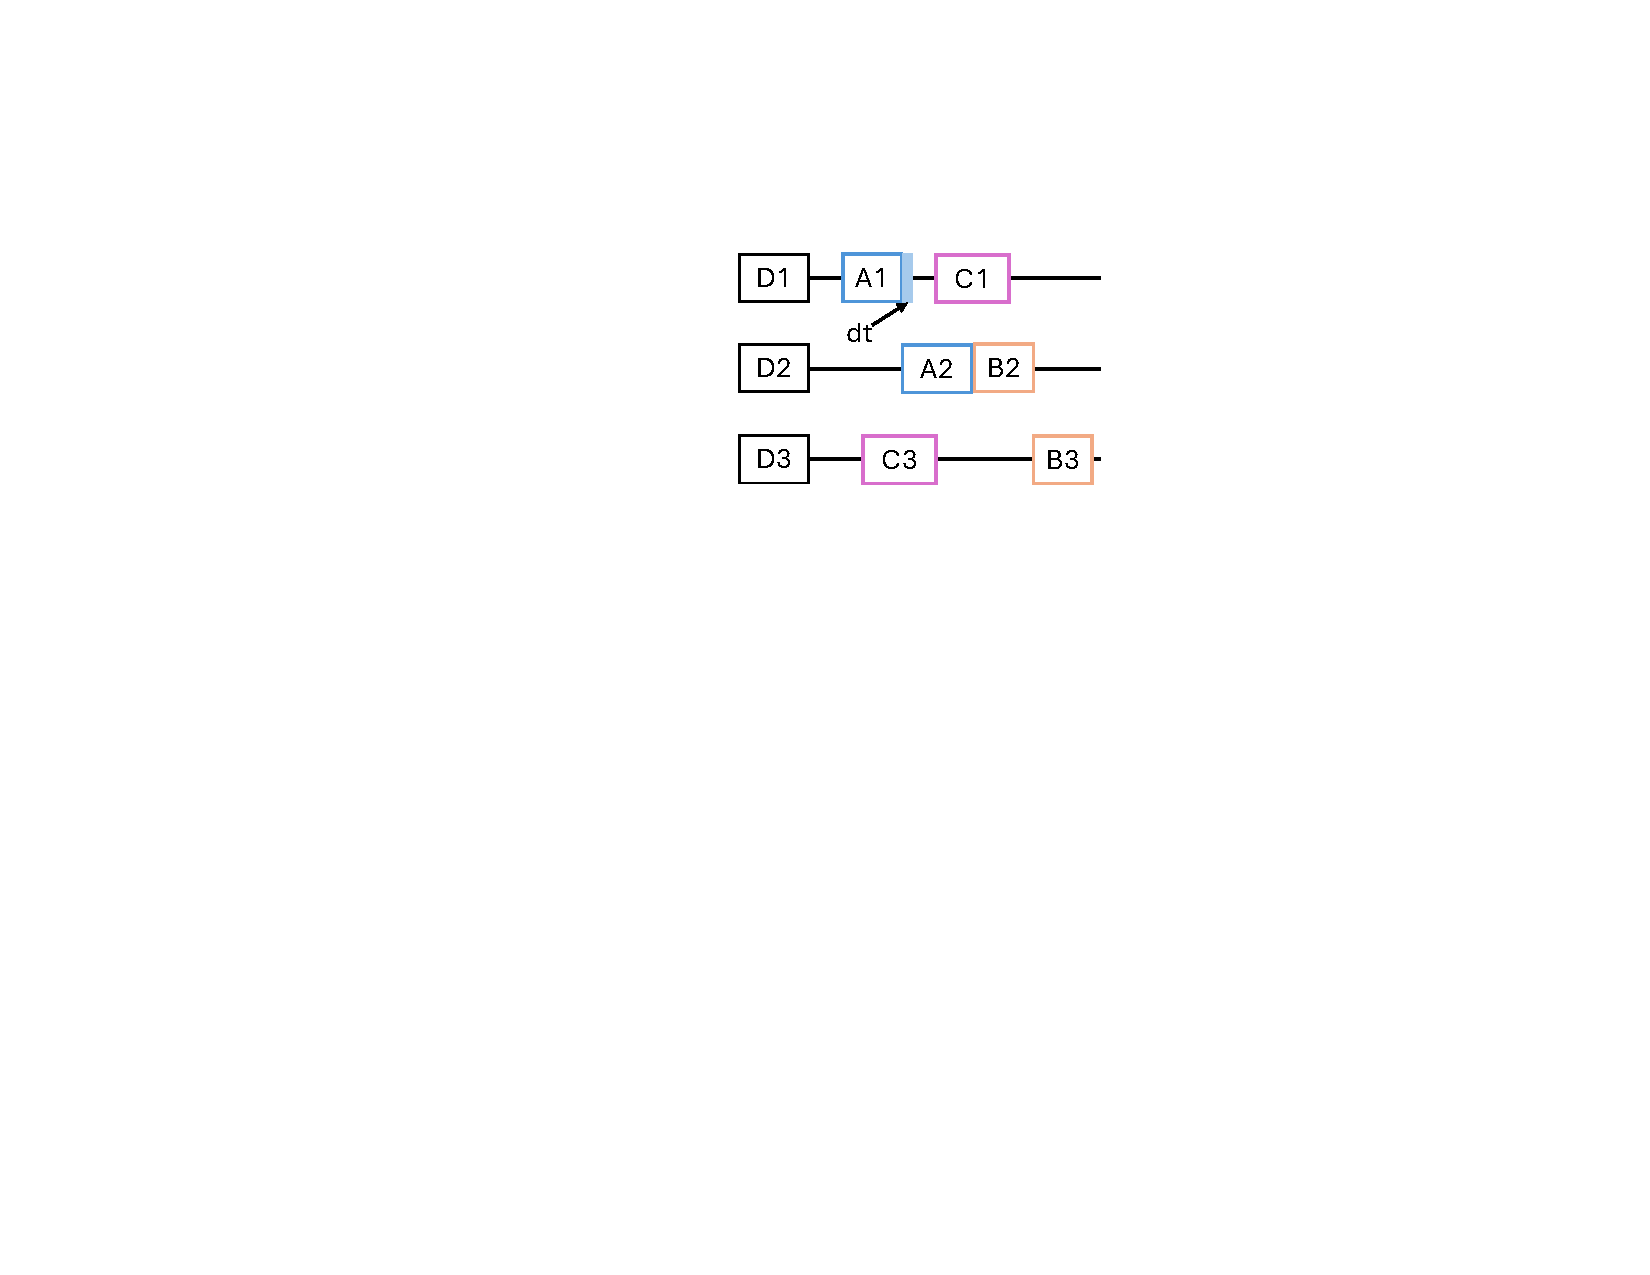
\includegraphics[width=\linewidth]{RASC/figures/applications/RASCal RV c.pdf}
        \caption{\small $A_1$ completes early $\rightarrow$ only RV.}
        \medskip
        \label{rasc:fig:rv-early}
    \end{subfigure}
    \hfill
    \begin{subfigure}[t]{0.28\linewidth}
        \centering
        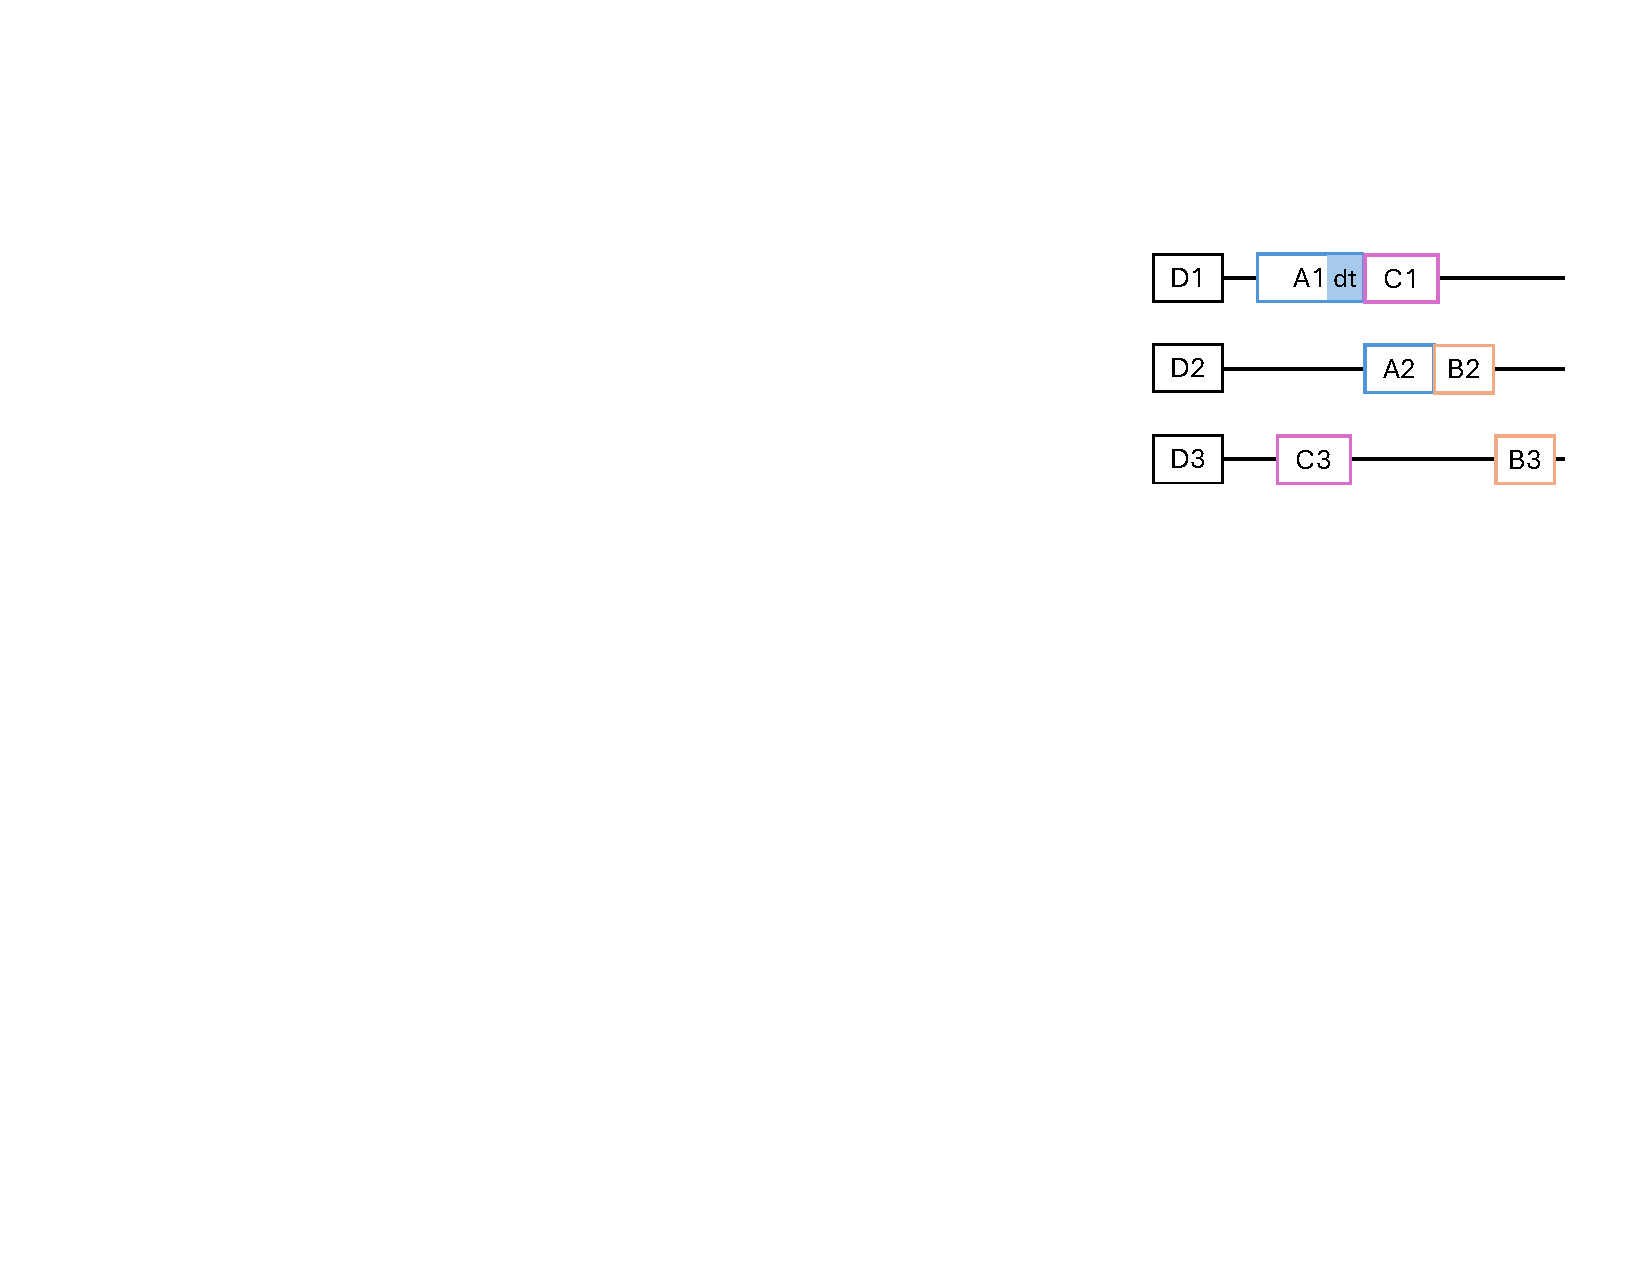
\includegraphics[width=\linewidth]{RASC/figures/applications/RASCal RV d.pdf}
        \caption{
            \small $A_1$ completes late $\rightarrow$ Push + RV.
        }
        \medskip
        \label{rasc:fig:rv-late}
    \end{subfigure}
    \caption{\bf \small RV rescheduling. {\it For (d), upon $A_1$'s late completion detection by an estimated $dt$, $C_1,A_2,B_2,B_3$ are first pushed forward by $dt$ before RV is performed.}}
    \medskip
    \label{rasc:fig:rv}
\end{figure}

Our second policy adapts \emph{Restriction Vectors (RV)} from real-time systems~\cite{manimaran1997new}.  
The classical RV pulls a task forward once all its parents finish to reclaim slack.
In \sysname{}, we apply this directly when progress points (e.g., \textit{Start}, \textit{Complete}) occur earlier than scheduled.
Unlike classical real-time settings, IoT actions may also finish \emph{later}, which is acceptable; to remain correct, we extend RV as follows:
(i) shift \textit{all} subsequent, not-yet-started actions forward by the observed delay to preserve safety; then
(ii) apply RV to the shifted schedule to exploit remaining slack.
Thus, RV stays correct under delays while still harvesting early-completion gains (see \Cref{rasc:fig:rv}).

\begin{theorem}[Action Safety]
\label{rasc:thm:safety}
For any device $D$, \sysname{}: (i) never initiates $>1$  action to $D$ concurrently, and  (ii) initiates an action only if $D$ is idle. Thus, ack-ed actions on $D$ execute in isolation.
\end{theorem}
\begin{proof}
\emph{\scheduler} assigns each action to the earliest idle slot on $D$ that respects dependencies.  
\emph{RV} may move actions earlier, but only when $D$ is idle and all parents are complete.
\emph{STF} inserts each action into the earliest idle slot consistent with serialization. Neither rule permits overlapping initiations.  
Thus, the non-overlap invariant is preserved under both schedulers and all rescheduling steps.
\end{proof}

\begin{theorem}[Serial Equivalence]
\label{rasc:thm:serial}
For any set of concurrent routines $\mathcal{R}$, the schedule $\mathcal{S}$ produced by \sysname{} is equivalent to executing $\mathcal{R}$ in some serial order $\pi(\mathcal{R})$.
This holds for the baseline scheduler and for rescheduling under RV and STF.
\end{theorem}
\begin{proof}
\emph{\scheduler} enforces a partial order $\prec$ on conflicting routines and produces a schedule $\mathcal{S}$ that extends $\prec$.
\emph{RV} 
advances or delays an action's start $s(a)$ only if $\prec$ is preserved.
\emph{STF} places each action $a$ in the earliest idle slot $i(a)$ consistent with $\prec$.
No step moves an action past the serialized prefix of a conflicting routine;
thus, $\mathcal{S}$ is equivalent to some serial order $\pi(\mathcal{R})$ consistent with $\prec$.
\end{proof}
